%!TEX root = ../../main.tex

\chapter{Fabrication of Nanodiamonds}	\label{ch::fabrication_nanodiamonds}
\chaptermark{Fabrication of Nanodiamonds}

	"Diamond forms under high temperature and pressure conditions that exist only about 100 miles beneath the earth’s surface." (Homepage of the Gemological Institute of America Inc.)
	While this statement is true for natural gem diamonds, various methods exist to synthetically produce diamond for applications in industry and research. 
	In this chapter, different fabrication methods of \nds are explained.
	The first two procedures described are the \hpht method and the \cvd are described.
	These are the most commonly used fabrication methods for laboratory-produced diamonds. 
	The \hpht (\HPHT) process is similar to the natural growth process within earth and is widly used to synthetically produce diamonds for industry.
	Many measurements which are subject in this thesis are carried out on diamond produced with a \CVD process. 
	The third method mentioned is the wet-milling in a vibrational mill.
	The main focus of this thesis is on wet-milling \nds, which is a technique using \cvd or \HPHT diamond as starting material. 
	It has to be stressed, that in contrast to the other methods described in this chapter, the wet-milling process is not a process to produce diamond itself, rather it serves to crush a bigger diamond into pieces of  a desired size.
	For a more extensive list of diamond production processes refer for example to \cite{davis1993diamond}.
	Aside from the diamond production processes, the technical details of the \nds used for this thesis will be mentioned.
	% At the end, the methods of producing diamonds via detonation processes and sonicating graphite powders are briefly described.
	% As diamonds produced with this process is not scope of this thesis, they will only be shortly introduced to complete the list.

	

	\section{High-Pressure High-Temperature Diamond}

	The \HPHT process was the first process with which diamond was successfully synthesized (in 1879).
	Depending on the exact process, temperatures and pressures are needed of a few thousand degrees Celsius and  \num{50000} to a few \num{100000}, respectively \cite{davis1993diamond}.
	Today, it is still widely used due to the relatively cheap production costs\cite{wikiSyntheticDiamond}.
	In this process, diamond is synthesized from graphite.
	For some forms of this method, a metallic solvent is added which lowers the needed pressures; the solvent causes the graphite to reach dissolve at lower pressures and temperatures, at the same time it causes the diamond to crystallize.
	The machine used for this kind of synthesis is a press.
	There exist several press designs, but they all provide a high temperature and a high pressure in their core.
	A disadvantage of the \HPHT process is that it the reachable size of the produced diamonds is limited.
	\todo{vorteile, nachteile}
	\todo{mention implanted NDs and Davidoff NDs}


	\section[CVD]{Chemical Vapor Deposition Diamond}

	\begin{figure}[tp]
		\begin{subfigure}[t]{ 0.49\linewidth}
			\caption{}\label{subfig::cvd_large}
			\centering
			\testbox{\includegraphics[trim = 0 0 0 0,  clip= true, height=5cm]{./pics/M05-13_191_131209_06.png}}
			% \caption{SEM picture of the milled nanodiamonds of a mean diameter of \SI{100}{\nano\meter}}
		\end{subfigure}
		\hfill
		\begin{subfigure}[t]{ 0.49\linewidth}
			\caption{}\label{subfig::cvd_detail}
			\centering
			\testbox{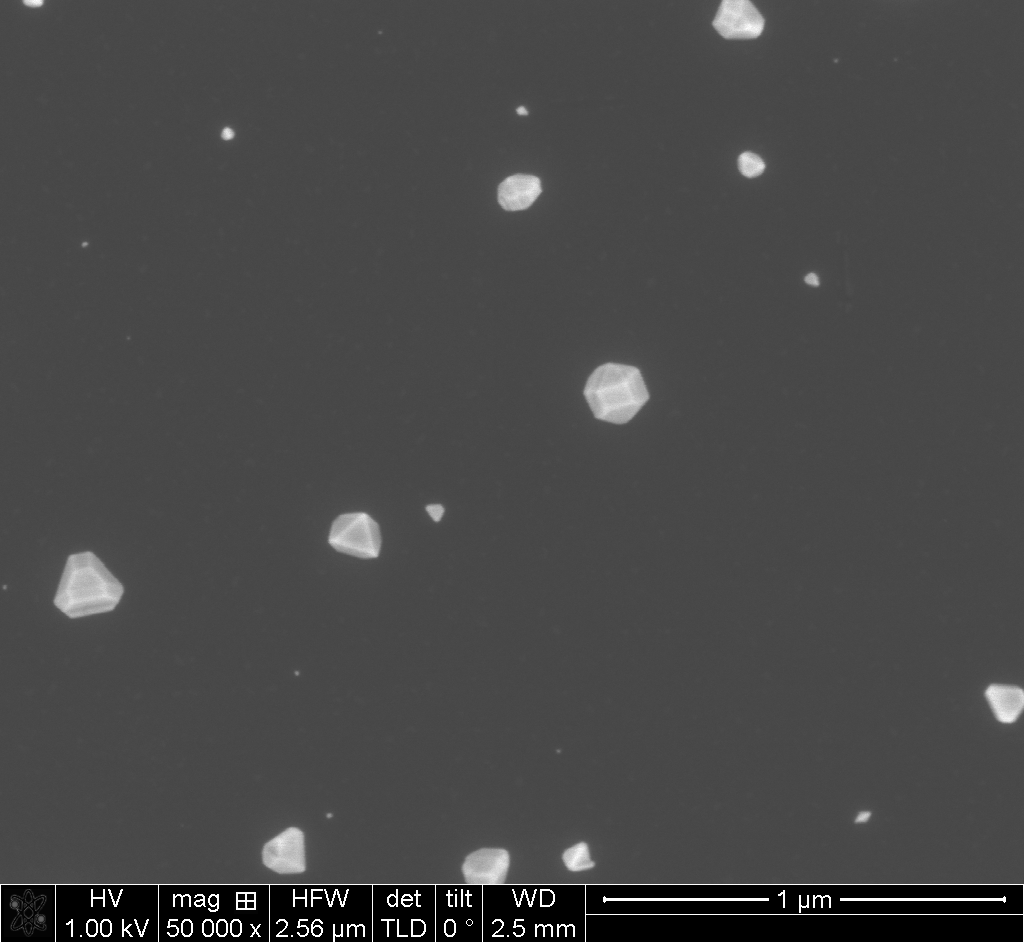
\includegraphics[trim = 0 0 0 0,  clip= true, height=5cm]{./pics/M05-13_191_131209_05.png}}
			% \caption{TEM picture of a \SI{100}{\nano\meter} diamond crystal.}
		\end{subfigure}
		\caption{}
		\label{fig::sem_cvd}
	\end{figure}

	\begin{figure}[tp]
		\centering
		\testbox{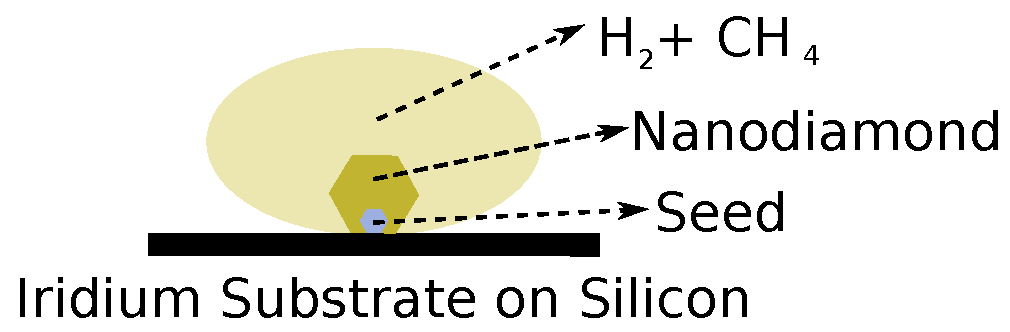
\includegraphics[trim = 0 0 0 0,  clip= true, width = 0.3\textwidth]{./pics/cvd_sketch.pdf}}
		\caption{Sketch showing the production of \CVD nanodiamonds in the growth chamber with a methane gas environment.}
		\label{fig::cvd_sketch}
	\end{figure}

	In contrast to the \HPHT process,  during the \cvd process, diamond is grown from a vapor phase.
	This process happens at moderate temperatures (\SIrange{700}{1300}{\celsius}) but very low pressures of less than 1 atmosphere in a vacuum chamber \cite{}
	The diamond grows outside its stability zone and atomic hydrogen is necessary to suppress the simultaneous growth of graphite.
	The vapor phase within the growth chamber is a mixture of hydrogen and methane, the latter of which acts as a carbon source.
	Within the vacuum chamber, activation of the gas by an energy source (e.g. microwave plasma) breaks apart the gas molecules to release carbon atoms. 
	These atoms are drawn down toward the cooler substrate.
	On the substrate surface, various processes occur, such as adsorption, desorption and diffusion.
	\\
	For crystals to form, initially diamond nuclei are necessary.
	The easiest method to obtain nuclei is to spin-coat a substrate with small diamond seed crystals of a size of a few nanometers. 
	This method is exploited for the production processes described in this section.
	Such small dimaond crystals are commercially available, and are usually diamond particles produced by a detonation process.
	For these detonation diamond seeds, the high pressure produced by shockwaves due to a detonation is used to form very small diamond particles of a size domn to a few nanometers.
	Growth on a substrate is easier, if the lattice constant of the substrate and the crystal to be grown are very similar.
	The lattice constant of \ir (\SI{0.384}{nm}\cite{Arblaster2010}) is very similar to the lattice constant of diamond (\SI{0.356}{nm}\cite{Davis1993}).
	Therefore, the diamonds were grown on a stratified substrate, consisting of \ir layers of \SIrange{60}{150}{nm} thickness grown onto an yttria-stabilized zirconia (YSZ) buffer layer, which in turn was grown on a silicon wafer.

	% There are two major different ways to make a plasma from the gas in the chamber: microwaves or a hot filament.
	% While the hot filament is easy to be technically implemented, it has the disadvantage that atoms which are etched from the filament during the growth process is likely to contaminate the diamond.
	% This circumstance can mess up a clean signal from \sivs.
	% Therefore, we preferred diamonds grown with in a microwave plasma.

	To produce \nds, the growth process is stopped when the diamond grown on the seed crystals reaches the desired size. 

	One of the advantages of the \CVD process is that \si can be incorporated \textit{in-situ}.
	This is achieved by the following process: \si from the substrate edges is etched by the \verify{plasma} and \si atoms diffuse into the methane gas. 
	These atoms are then build into the diamond lattice while growth.
	\\
	In this thesis, two types of samples which were directly produced as nanodiamonds were investigated.
	The first batch (henceforth called \CVD samples) were grown on detonation diamond seeds (produced by the company Microdiamant, product Liquid Diamond monocrystalline, MSY 0-0.03 micron GAF) of a size smaller than \SI{3}{nm}.
	For the growth process, 1\% of methane was added to the hydrogen environment in the growth chamber.
	The growth process was performed with a pressure of \SI{30}{hPa} for \SIrange{30}{60}{min}, yielding \nds of a diameter of about \SIrange{100}{200}{nm}.
	\todo{put in figure}
	\\
	The other samples solely produced by a \CVD process are nanodiamonds grown onto molecular analogs of diamond crystals.
	A subgroup of these molecular diamonds are called diamondoids and are carbon crystals based on the carbon cage molecule adamantane \ch{C10H16}.
	The molecular diamonds used for this work are adamantane in cyclohexane, mercapto adamantane in cyclohexane, and cyclohexane.
	Each of these seed crystals was used in different growth processes.
	During the growth process, either 3\% or 1\% methane was added to the hydrogen plasma and either \si or \si dioxide was exploited to form \textit{in-situ} incorporated \sivs (see \autoref{tab::diamondiods}).


	\begin{table}[tp] 
		\centering 
		\caption{Summary of the samples grown on diamondoid seed crystals.} \label{tab::diamondiods} 
			\begin{tabular}{llll} 
			\toprule
			Sample name & Seed crystals & Methane conc. & \Si source \\ 
			\midrule
			160211\_E & Mercapto adamentane in cyclohexane & 1\% & \ch\{SiO2\} \\
			160211\_F & Cyclohexane                        & 1\% & \ch\{SiO2\} \\
			160212\_C & Cyclohexane                        & 3\% & \si         \\
			160212\_D & Adamentane in cyclohexane          & 3\% & \ch\{SiO2\} \\
			160212\_E & Mercapto adamentane in cyclohexane & 3\% & \ch\{SiOs\} \\
			160212\_F & Cyclohexane                        & 3\% & \ch\{SiO2\}\\
			\bottomrule
			\end{tabular} 
	\end{table}






	\section{Wet-Milled Nanodiamonds}
	% \section{Detonation and Sonification Processes}

	\begin{figure}[tp]
		\begin{subfigure}[t]{ 0.49\linewidth}
			\caption{}\label{subfig::sem_milled}
			\centering
			\testbox{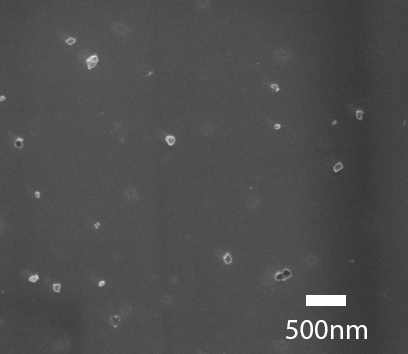
\includegraphics[trim = 0 0 0 0,  clip= true, height=5cm]{./pics/Ir27M_mitte_213_151111_22_crop.jpg}}
			% \caption{SEM picture of the milled nanodiamonds of a mean diameter of \SI{100}{\nano\meter}}
		\end{subfigure}
		\hfill
		\begin{subfigure}[t]{ 0.49\linewidth}
			\caption{}\label{subfig::tem_milled}
			\centering
			\testbox{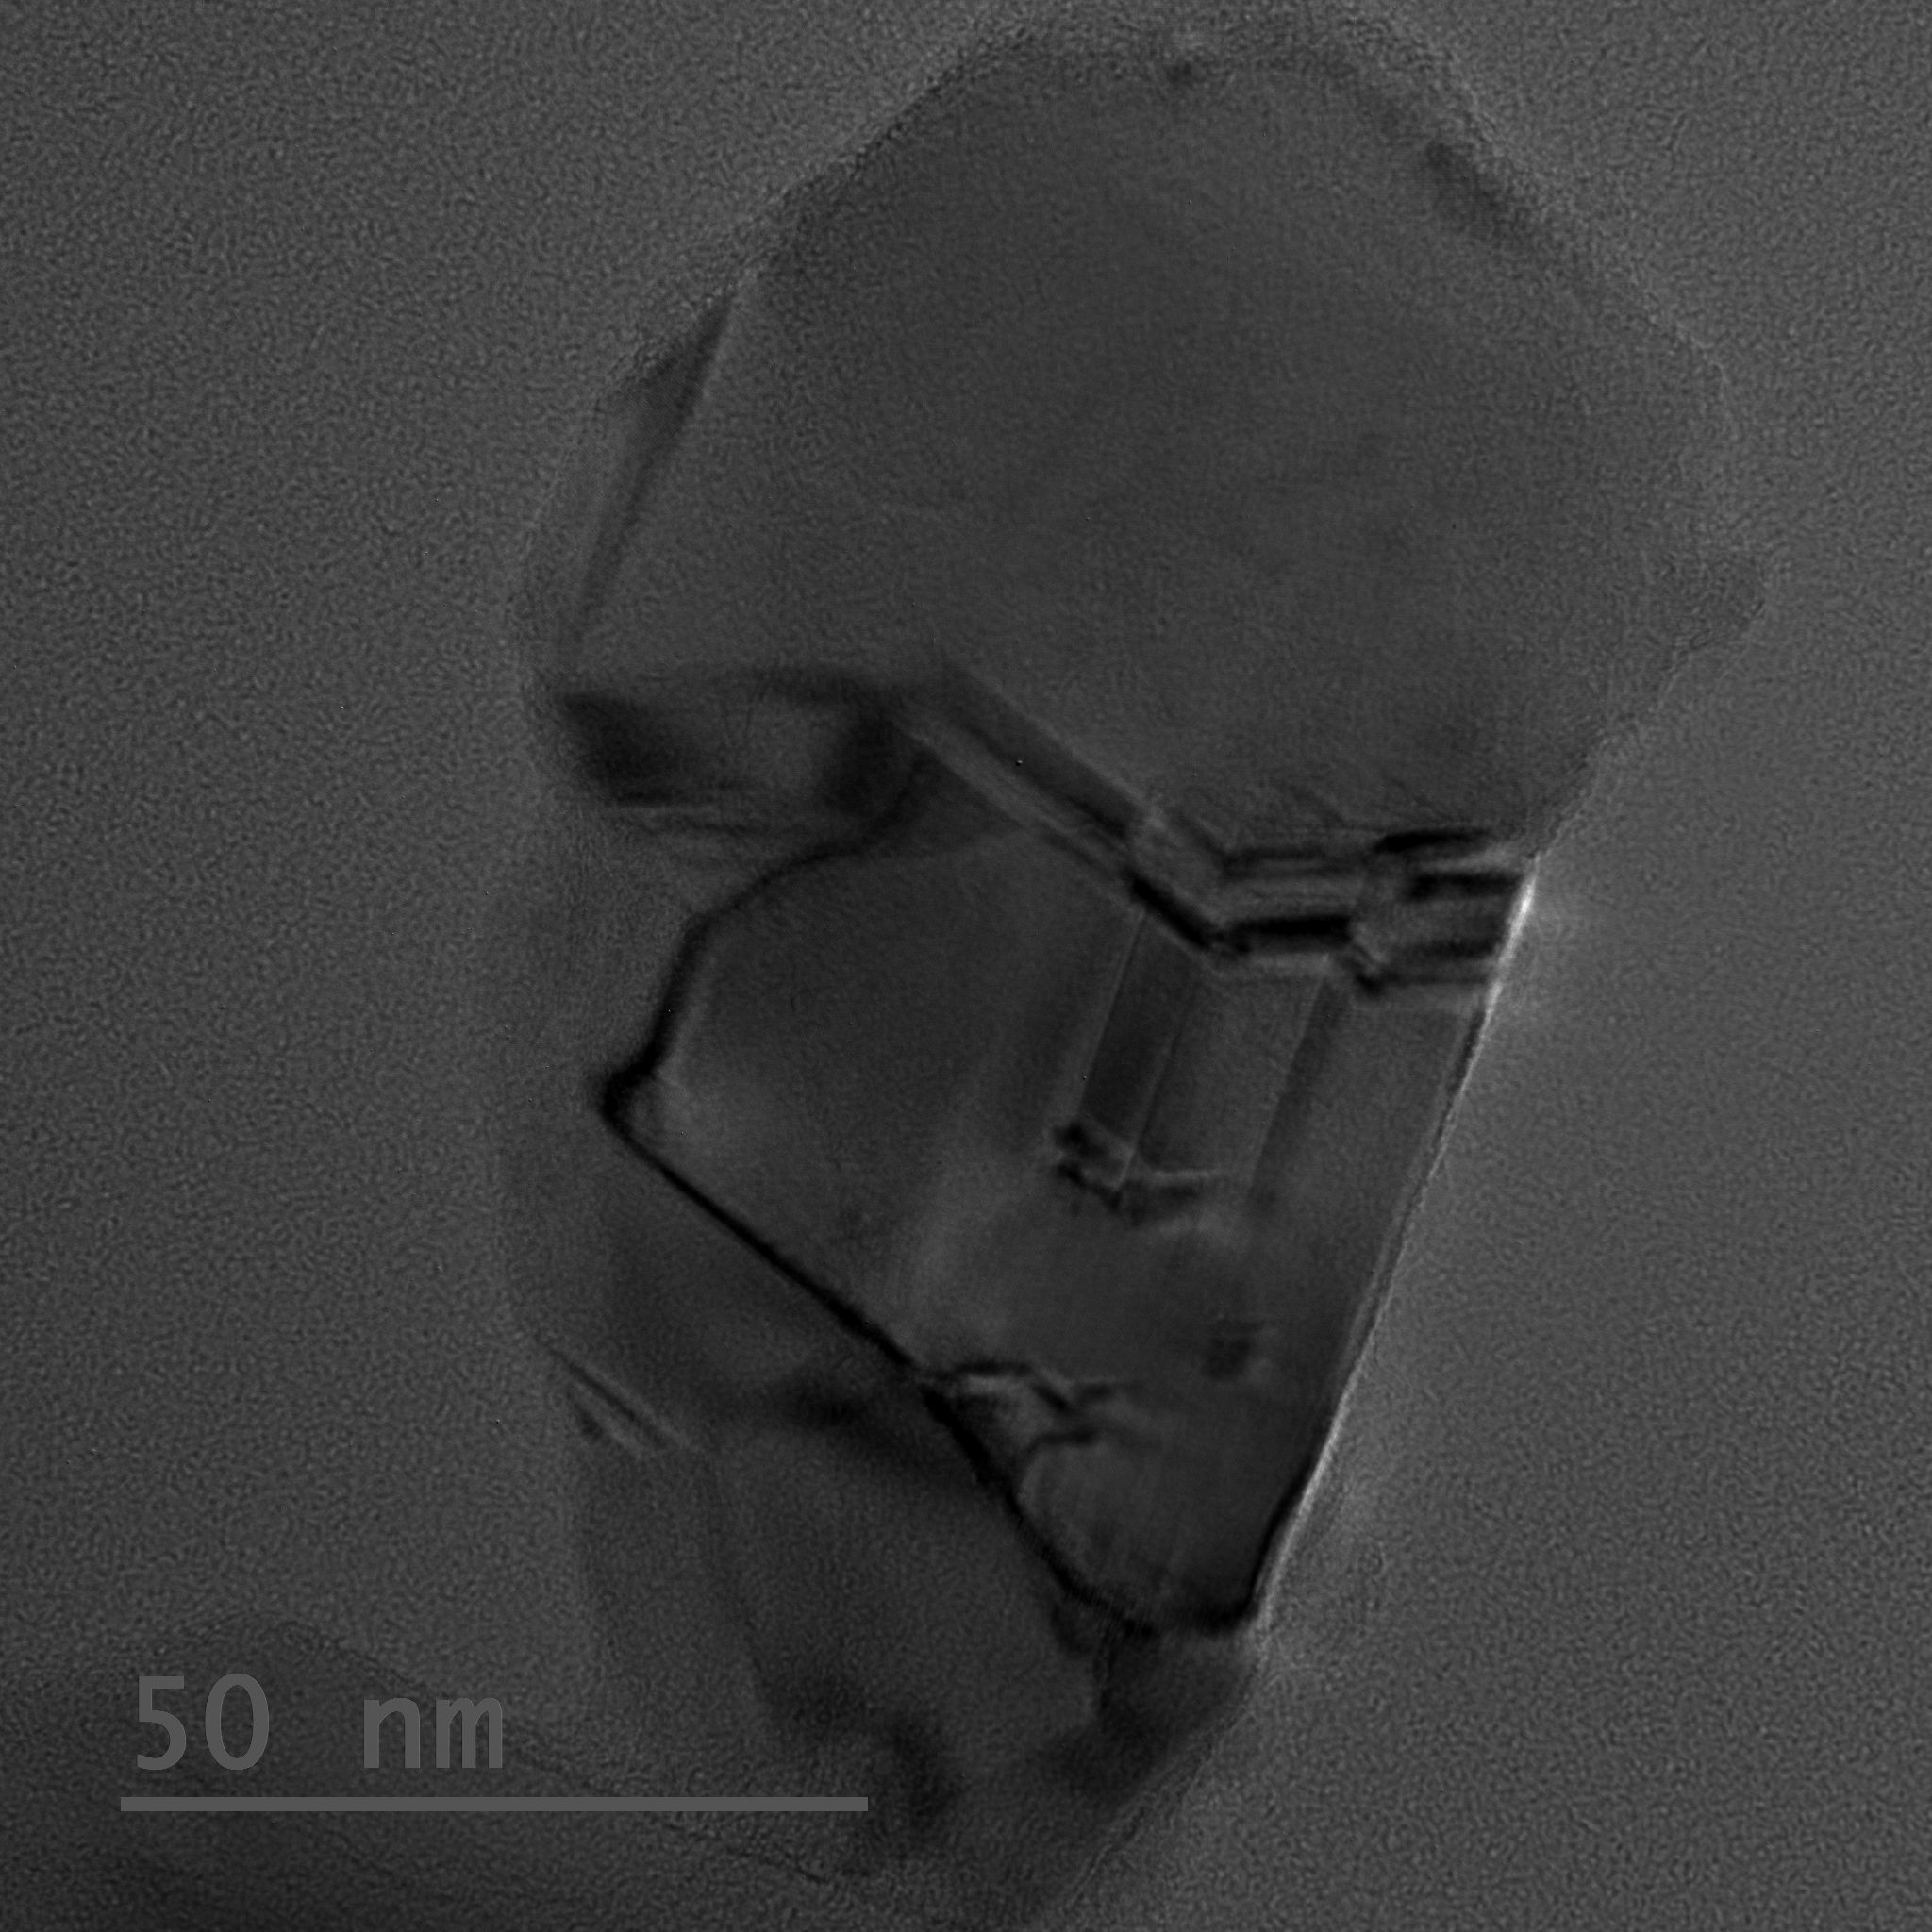
\includegraphics[trim = 0 0 0 0,  clip= true, height=5cm]{./pics/AM060-II-k4-2.png}}
			% \caption{TEM picture of a \SI{100}{\nano\meter} diamond crystal.}
		\end{subfigure}
		\caption{Pictures of the milled \nds (sample \insituH). (a) SEM picture showing the distribution of the \nd crystals on the \ir substrate. (b) TEM picture of a \nd particle.}
		\label{fig::semtem_millled}
	\end{figure}

	\begin{figure}[tp]
		\centering
		\testbox{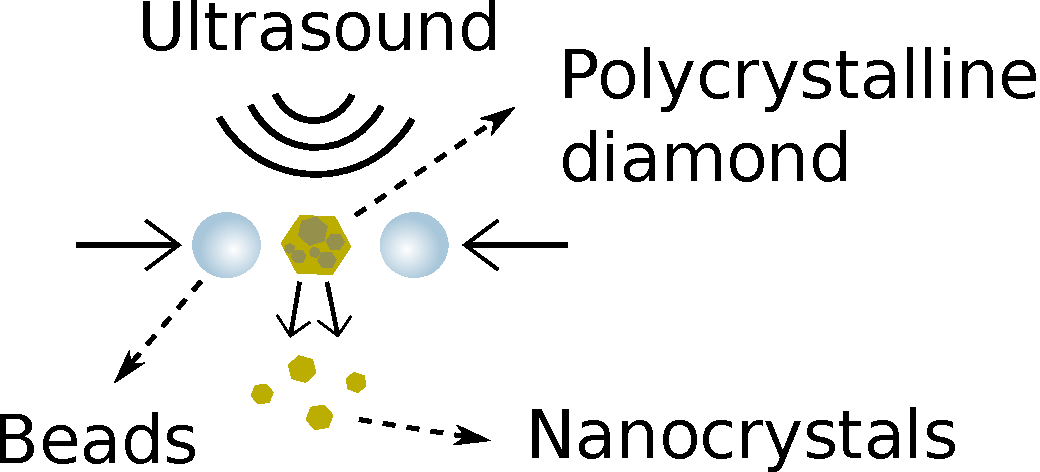
\includegraphics[trim = 0 0 0 0,  clip= true, width = 0.3\textwidth]{./pics/basd_sketch.pdf}}
		\caption{Sketch showing the \basd process. In a vibrational mill, vibrations from the mill drive the beads instead of the ultrasonic waves.}
		\label{fig::sketch_basd}
	\end{figure}

	Apart from growing \nds of a specific size directly via a \CVD process, macroscopic diamond starting material can be crushed to obtain small diamond particles.
	As starting material, both \HPHT diamond and \CVD grown diamond films are used.
	There are two major milling procedures: \basd (\BASD) and wet-milling in a vibrational mill.
	Both techniques use small beads to crush the diamond material. 
	The beads are either driven by ultrasonic waves (in the \BASD process) or by vibrations of the vibrational mill\todo{info about vibrational mill}.
	A sketch of the process is shown in \autoref{fig::sketch_basd}.
	\\
	In the following paragraphs, details of the production processes of the investigated wet-milled samples are described. 
	For an overview of the samples refer to \autoref{tab::samplenames}.
	The starting material for the wet-milled \nds was a nanocristalline diamond film \cite{Williams2006a} directly grown on a silicon wafer by chemical vapor deposition (CVD). 
	A microwave hydrogen plasma containing 1\% methane was used to grow on purified \SI{5}{\nano\meter} nanodiamond seeds (produced by PlasmaChem).
	To induce \textit{in-situ} \siv creation, sacrificial \Si pieces are situated in the growth chamber.
	During diamond growth the \Si pieces are etched by the plasma and individual atoms are incorporated into the diamond lattice.
	The diamond film is then milled by a wet-milling process in a vibrational mill with steel beads to crystals of average diameters of \SIlist{50; 70; 100}{\nano\meter} (\autoref{subfig::sem}).
	The particle size was determined with laser diffraction spectroscopy.
	Transmission Electron Microscopy (TEM) pictures of the diamond crystals show that the milled \nds are polycristalline, exhibiting a typical size of single crystals of a few tens of nanometers.
	In \autoref{subfig::tem} a TEM image of a typical \nd is shown.
	Crystal boundaries have effects on the formation of color centers:
	\sivs are more prone to form at crystal boundaries \cite{Zapol2001}.
	The high amount of steel containment due to the steel beads is removed by extensive acid treatment.
	We also investigated \nds milled with silicon nitride beads, and found that the choice of material of the beads did not cause any spectroscopic difference.
	The aqueous solution containing the \nds is drop cast onto an \ir film on a \Si substrate.
	The \ir film of a thickness of \SI{130}{nm} is grown onto a buffer layer of yttria-stabilized zirconia (YSL) whith in turn is grown onto a \Si wafer.
	The \ir surface has the advantage that it acts as an antenna and therefore enhances the collection efficiency of fluorescence light \cite{Neu2012a}.
	Prior to drop casting, the substrate was cleaned in Piranha solution (50\% sulfuric acid H$_2$SO$_4$, 50\% hydrogen peroxide H$_2$O$_2$) to enhance the surface hydrophilicity and therefore obtain a homogeneous distribution of diamonds on the surface.
	Post-procession treatment comprises either both annealing in vacuum at \SI{900}{\degreeCelsius} and consecutive \ox in air at a temperature of \SI{450}{\degreeCelsius}, or only one of the two methods.
	The duration for either treatment method was 3-6 hours.
	\\
	For comparative measurements, we also investigated \nds with \sivs implanted after diamond growth. 
	For those \nds starting material was a polycristalline Element Six diamond film (electronic grade).
	In bulk material, the implantation causes the \sivs to form in a specific depth dependent on the implantation energy, leaving most of the diamond vacant of \sivs.
	As a consequence, a big portion of  \nds milled from such a bulk material would not host any \sivs.
	To obtain diamond particles with a homogeneous distribution of \sivs, the implanted \nds are produced in several steps. 
	First, the diamond film was milled to diamond particles of sizes of a few micrometers.
	In the second step, these microdiamonds were then densely spin-coated onto \ir substrates and implanted with \si (implantation energy \SI{900}{keV}, fluence \SI{e11}{\per\centi\meter\squared}).
	To eliminate damage from the implantation process, the diamonds were annealed in vacuum at \SI{900}{\degreeCelsius} for 3 hours and subsequently oxidized in air at \SI{450}{\degreeCelsius} also for 3 hours.
	At last, the micrometer sized diamond particles were milled to a size of \SI{250}{\nano\meter}.


	\begin{table}[tp] 
		\centering 
		\caption{Summary of the wet-milled samples. The first column indicates the names of the samples, the second the mean diameter of the \nds, and the third describes how the \si was incorporated into the diamond.} \label{tab::samplenames} 
			\begin{tabular}{llll} 
			\toprule
			Sample name & Size & Si incorporation & Post-processing \\ 
			\midrule
			\insituF & \SI{50}{nm} & \textit{in-situ} & \begin{tabular}[c]{@{}l@{}}series of individual samples \\ with diverse post-processing steps\end{tabular}\\ \hline 
			\insituS & \SI{70}{nm} & \textit{in-situ} & \begin{tabular}[c]{@{}l@{}}series of individual samples \\ with diverse post-processing steps\end{tabular}\\ \hline 
			\insituSn & \SI{70}{nm} & \textit{in-situ} &  \begin{tabular}[c]{@{}l@{}}no post-processing \\ subset of \insituS \end{tabular}\\ \hline 
			\insituSo & \SI{70}{nm} & \textit{in-situ} & \begin{tabular}[c]{@{}l@{}}oxidized in air at 450\textdegree C \\ subset of \insituS \end{tabular}\\ \hline 
			\insituH & \SI{100}{nm} & \textit{in-situ} & \begin{tabular}[c]{@{}l@{}}series of individual samples \\ with diverse post-processing steps\end{tabular}\\ \hline 
			\insituHao & \SI{100}{nm} & \textit{in-situ} & \begin{tabular}[c]{@{}l@{}}annealed in vacuum at 900\textdegree C, \\ consecutively oxidized in air at 450\textdegree C \\ subset of \insituH \end{tabular}\\ \hline 
			\implantedTao & \SI{250}{nm} & implanted & \begin{tabular}[c]{@{}l@{}}annealed in vacuum at 900\textdegree C, \\ consecutively oxidized in air at 450\textdegree C\end{tabular}\\ 
			\bottomrule
			\end{tabular} 
	\end{table}

